%*============================================================*
%**Goal		:    文献分享:Long-Term Effects Of The 1959-1961 China Famine: Mainland China and Hong Kong
%**Author	:  	 ZhangYi zhangyiceee@163.com 15592606739
%**Created	:  	 20200513
%**Last Modified: 2020
%*============================================================*



\documentclass{beamer}
\usepackage[UTF8,noindent]{ctexcap}
\graphicspath{{figures/}}


\usetheme{Madrid}
%Information to be included in the title page:
\title[文献分享:ZY]{Long-Term Effects Of The 1959-1961 China Famine: Mainland China and Hong Kong}
\author[Famine\_workshop]{Douglas Almond、Lena Edlund、Hongbin Li \&Junsen Zhang}
\date{\today}

\begin{document}
\frame{\titlepage}
%开始你的表演


\begin{frame}
	\frametitle{Abstract}
This paper estimates the effects of maternal malnutrition exploiting the 1959-1961 Chinese famine as a natural experiment. In the 1\% sample of the 2000 Chinese Census, we find that fetal exposure to acute maternal malnutrition had compromised a range of socioeconomic outcomes, including: literacy, labor market status, wealth and marriage market outcomes. Women married spouses with less education and later, as did men, if at all. In addition, maternal malnutrition reduced the sex ratio (males to females) in two generations -- those prenatally exposed and their children -- presumably through heightened male mortality. This tendency toward female offspring is interpretable in light of the Trivers-Willard (1973) hypothesis, according to which parents in poor condition should skew the offspring sex ratio toward daughters. Hong Kong natality micro data from 1984-2004 further confirm this pattern of female offspring among mainland-born residents exposed to malnutrition in utero.
\end{frame}

\begin{frame}
	\frametitle{Problem}
Evidence on the causal effects of fetal nutrition, however, is surprisingly scarce.

\end{frame}


\begin{frame}
	\frametitle{1.1 Introduction:Background}
1959年秋季开始的饥荒影响整个中国全境,导致粮食减产,一直持续到1962年出生和死亡率才恢复正常。有很多原因:天灾、人祸(大跃进被认为是主因)

\end{frame}


\begin{frame}
	\frametitle{Introduction Famine studies}
	分为两个部分:流行病学研究和经济学研究
	\begin{itemize}
		\item 流行病学:针对健康的Y变量
		\item 经济学:对生存者的社会经济产出的影响(CHNS),但是存在一些缺点。
	\end{itemize}
\end{frame}


\begin{frame}
	\frametitle{2:Data}
	数据1:2000年1\%人口普查的数据,Y变量:受教育程度、职业地位、居住信息、个体特征(性别、出生年月、婚姻和生育信息)
	\\数据与CHNS的不同点在于减少了一些混杂因素:迁移,2000年普查数据优势多,将样本限制在1956-1964年间,饥荒前三年和后三年
	\\数据2:香港1984-2004年出生记录的微观数据:包含母亲出生的城市,将样本限制在1957-1965年出生在香港或者大陆的单身母亲(600000个样本),1/3的样本来自大陆,香港的样本提供了一个很好的对照组,因为大陆全境在当时都遭受了饥荒。
\end{frame}



\begin{frame}
	\frametitle{2.1 Measuring the Famine}
\begin{itemize}
	\item 死亡率(Death rate):根据2000年的普查数据有各省各年各年龄段的死亡数据,构建两个变量以代表饥荒的严重程度。加权死亡率(Weighted death rate)$wdr_{jt}$例子:一个1960年1月出生在北京的人:分配到1/9的1960年的北京死亡率+8/9的1959年北京死亡率(从怀孕到出生9个月)
	\item 总加权死亡率$awdr_{t}$ we collapse this weighted death rate by month of birth, thus calculating a population weighted national average for each month and year, henceforth “aggregate weighted death rate” 
	\item 平均月出生率
\end{itemize}
\end{frame}


\begin{frame}
\frametitle{Result:Descriptive Results}
	\begin{columns}
            \column{0.6\textwidth}
            \begin{minipage}[c][0.4\textheight][c]{\linewidth}
                \centering
                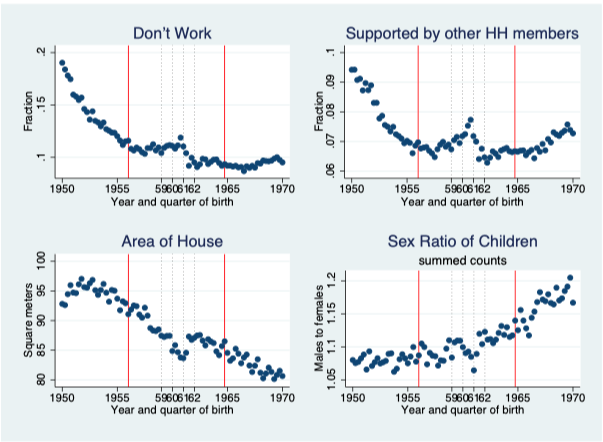
\includegraphics[width=0.9\linewidth]{figure5}
            \end{minipage}
           
            \column{0.4\textwidth} % remember add this to the other clumn
           	\begin{minipage}[c][0.4\textheight][c]{\linewidth}
            2000年的统计微观数据显示:在1960年前后出生的人,与同期预测相比有更差的社会经济产出。
            在1960年出生的人在2000年普查时特征:没有工作;受其他家庭成员支持;住在很小的地方;女童的父母
            \end{minipage}
    \end{columns}
\end{frame}

\begin{frame}
	\frametitle{Result:Regression Results}
	$$y_{it}=\beta_0+\theta~awdr_t+\beta_1YOB+\beta_2YOB^2+\beta_3YOB^3+\lambda_{province}+\varepsilon_{it}$$
	$y_{it}$代表t时期出生的i个体的结果变量,$awdr_t$表示按出生年份和出生月份计算的总加权死亡率;$YOB$出生年份,加入平方和立方项控制非线形趋势(图五的四幅图);$\lambda_{province}$省的虚拟变量,由于出生月份存在明显的内生性,所以不包括月份的虚拟变量
\end{frame}


\begin{frame}
\frametitle{Result:Regression Results}
	\begin{columns}
            \column{0.6\textwidth}
            \begin{minipage}[c][0.4\textheight][c]{\linewidth}
                \centering
                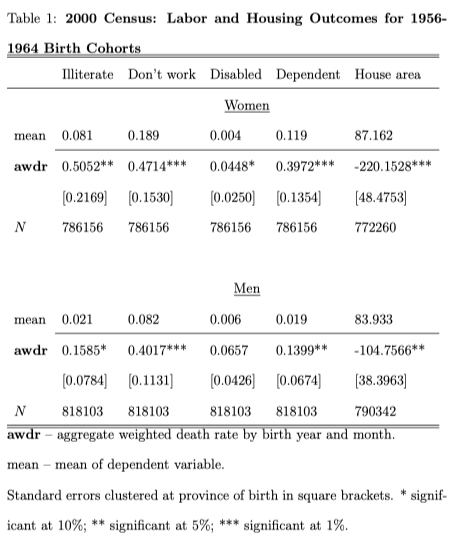
\includegraphics[width=0.9\linewidth]{table1}
            \end{minipage}
           
            \column{0.4\textwidth} % remember add this to the other clumn
           	\begin{minipage}[c][0.4\textheight][c]{\linewidth}
            Greater famine intensity is associated with a higher likelihood of being illiterate and not working.\\awdr提高1.2个百分点,意味着:饥荒经历的女性有$0.502*0.012/0.081=7.5\%$的可能性是文盲,但是这个普查的数据没有其他直接的关于收入的数据
            \end{minipage}
    \end{columns}
\end{frame}

\begin{frame}
\frametitle{Result:Regression Results}
	\begin{columns}
            \column{0.5\textwidth}
            \begin{minipage}[c][0.4\textheight][c]{\linewidth}
                \centering
                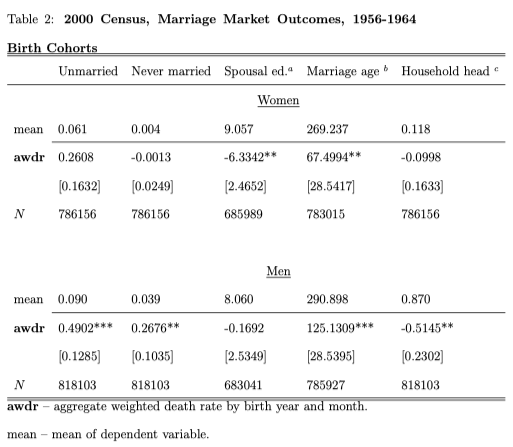
\includegraphics[width=1\linewidth]{table2}
            \end{minipage}
           
            \column{0.5\textwidth} % remember add this to the other clumn
           	\begin{minipage}[c][0.4\textheight][c]{\linewidth}
            表2主要研究对于婚姻市场的影响:对于女性而言不显著,但是女性更易的伴侣通常的教育程度更低,但是男性更易受到影响:未婚等,结婚年龄的影响,主要解释:婚姻市场挤压
            \end{minipage}
    \end{columns}
\end{frame}

\begin{frame}
\frametitle{Result:Regression Results}
	\begin{columns}
            \column{0.5\textwidth}
            \begin{minipage}[c][0.4\textheight][c]{\linewidth}
                \centering
                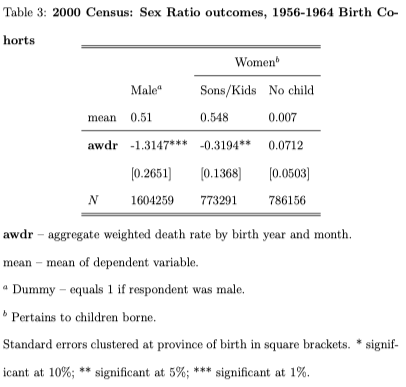
\includegraphics[width=1\linewidth]{table3}
            \end{minipage}
           
            \column{0.5\textwidth} % remember add this to the other clumn
           	\begin{minipage}[c][0.4\textheight][c]{\linewidth}
            男性死亡率提高,母亲经历过饥荒的越严重,后代中女性更多,因此需要香港数据进行验证
            \end{minipage}
    \end{columns}
\end{frame}

\begin{frame}
	\frametitle{Result:Geographic variation in Famine intensity}
    将饥荒的地域差异控制住,研究出生队列间的差异,这样会降低未来生活中其他因素与特定年龄混杂的可能性
$$y_{it}=\beta_0+\theta~wdr_t+\gamma_{yob}+\lambda_{province}+\varepsilon_{itj}$$


\end{frame}

\begin{frame}
	\frametitle{}
\end{frame}

\begin{frame}
	\frametitle{}
\end{frame}


\end{document}




